\chapter{FUNDAMENTAÇÃO TEÓRICA}

Este capítulo apresenta os principais conceitos teóricos que embasam o desenvolvimento deste trabalho, cuja proposta está inserida no contexto de teste de software em jogos digitais. Inicialmente, na Seção 2.1, é abordado o cenário dos jogos digitais no Brasil, destacando seu crescimento expressivo, relevância cultural e impacto econômico. Na Seção 2.2, discute-se o conceito de anomalias visuais em jogos digitais, suas categorias mais comuns, causas e implicações na experiência do usuário.

A Seção 2.3 introduz os fundamentos do \gls{am}, com foco nas \glspl{rna}, especialmente nas \glspl{cnn}, explorando suas arquiteturas, funcionamento e aplicações na detecção de padrões visuais. Na Seção 2.4, são apresentadas as principais métricas utilizadas para avaliar o desempenho de modelos baseados em \glspl{rna}.

A Seção 2.5 trata dos tipos de classificação em redes neurais, com ênfase nas abordagens binária e multiclasse. Na Seção 2.6 discute o processo de teste de software em jogos digitais, destacando seus desafios específicos e o potencial da automação por meio de técnicas de visão computacional. "Por fim, a Seção 2.7 apresenta os trabalhos correlatos, destacando pesquisas anteriores sobre o tema e situando a proposta no contexto científico atual.

\section{O cenário dos jogos digitais no Brasil} %completo

A indústria de jogos digitais tem se consolidado como um dos segmentos mais relevantes do mercado global de entretenimento. Representando uma forma de expressão cultural, artística e tecnológica, os jogos digitais atingem públicos de todas as idades e estão presentes em diversas plataformas, refletindo o avanço das tecnologias digitais na sociedade contemporânea (\citeonline{araujo2024produccao}). 

No Brasil, esse fenômeno tem ganhado proporções significativas, impulsionado pela popularização de dispositivos móveis, pelo aumento do acesso à internet e pela ampliação do consumo de conteúdos digitais. Segundo a \citeonline{abragames2022}, entre 2014 e 2022 o número de estúdios de desenvolvimento de jogos no Brasil aumentou de 133 para 1.009, evidenciando um crescimento de mais de sete vezes em menos de uma década. Esse avanço expressivo pode ser visualizado na Figura ~\ref{fig:estudios}, que ilustra claramente a evolução do número de estúdios no período analisado.

\begin{figure}[H]
    \centering
    \caption{Evolução do número de estúdios de desenvolvimento de jogos no Brasil}
    \vspace{0.5cm} % Espaço entre a imagem e a fonte
    
    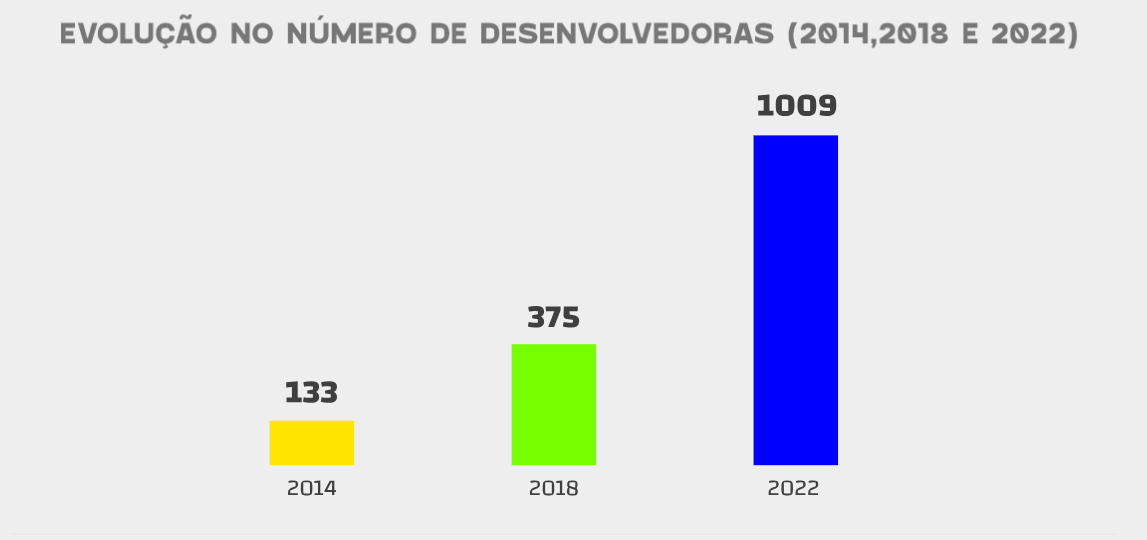
\includegraphics[width=12cm]{images/abragames.png}
    
    \vspace{0.5cm} % Espaço entre a legenda e a fonte
    
    {\small \textbf{Fonte:} \citeonline{abragames2022}}
    \label{fig:estudios}
\end{figure}

Segundo os dados da Pesquisa Game Brasil, "três em cada quatro pessoas no Brasil usam celulares, videogames ou computadores para jogar" (\citeonline{cnnbrasil2024}). Essa presença massiva reflete não apenas um crescimento no número de jogadores, mas também uma transformação no perfil do consumidor, que se mostra mais exigente em relação à qualidade gráfica, jogabilidade e performance dos títulos.

\section{Anomalias visuais em jogos digitais} % COMPLETO

O crescimento expressivo do público gamer no Brasil reforça a necessidade de experiências visuais cada vez mais refinadas e imersivas, o que evidencia a abrangência dos jogos eletrônicos como forma dominante de entretenimento. Conforme aponta \citeonline{backus2025investigating}, assim como qualquer outro software, os videogames estão sujeitos a erros que aparecem principalmente na forma de bugs e glitches. Embora distintos, esses termos são frequentemente confundidos pelos jogadores devido à complexidade envolvida.

Um bug é caracterizado como um erro interno do sistema que compromete o funcionamento adequado de certas mecânicas, como quando um jogador não consegue interagir com um objeto essencial. Já um glitch é uma falha que ocorre mesmo com os sistemas do jogo funcionando normalmente, afetando especialmente a aparência visual como por exemplo, quando objetos se sobrepõem ou atravessam cenários de maneira não natural, exatamente como descrito por \citeonline{backus2025investigating}.

\section{Machine learning} 

Machine Learning, ou Aprendizado de Máquina (\acrshort{am}), é um campo da inteligência artificial voltado ao desenvolvimento de algoritmos capazes de identificar padrões e tomar decisões com base em dados. Nessa perspectiva, segue a definição de \citeonline{rossi2015classificacao}:
\begin{citacao}
O objetivo dos algoritmos de aprendizado de máquina é aprender, generalizar, ou ainda extrair padrões ou características das classes das coleções com base nos documentos textuais e rótulos (identificadores de classe) dos documentos informados por um usuário ou especialista de domínio (\citeonline[p.~2]{rossi2015classificacao}).
\end{citacao}

Essa definição reforça a ideia de que, ao serem treinados com dados rotulados, os algoritmos conseguem construir modelos que reconhecem características relevantes e realizam previsões sobre novos dados.


Entre os diversos métodos utilizados no campo do Aprendizado de Máquina, um dos mais relevantes e amplamente adotados é o das Redes Neurais Artificiais (\glspl{rna}), que se destacam por sua capacidade de modelar relações complexas e não lineares entre os dados.

\subsection{Redes neurais artificiais}

As \glspl{rna} têm sua origem inspirada no funcionamento dos neurônios do cérebro humano. Elas são constituídas por um conjunto de neurônios artificiais que buscam simular a forma, o comportamento e as funções dos neurônios biológicos, o que permite às RNAs aprenderem e reconhecerem padrões de maneira semelhante ao sistema nervoso (\citeonline{borges2020aplicaccao}). Essa semelhança estrutural e funcional é fundamental para a aplicação das RNAs em diversas áreas, como reconhecimento de imagens, processamento de linguagem natural e previsão de séries temporais. Nesse contexto, destaca-se o seguinte trecho:

\begin{citacao}
As redes neurais artificiais (RNA) são definidas como processadores maciçamente paralelos que simulam o cérebro humano na intenção de coletar evidências empíricas e também à medida que preservam e permitem o uso do conhecimento experimental. Em seu funcionamento, existem sinapses (ou ligações inter-neurais) que são usadas para fins de aprendizagem e armazenamento do conhecimento. (Haykin, 1999, apud Santos et al., \citeyear{santos2016aplicaccao})

\end{citacao}

Essa definição ressalta a capacidade das \glspl{rna} de aprender a partir de exemplos, armazenando e generalizando padrões complexos de dados. Para entender como isso acontece, é fundamental compreender os elementos básicos que compõem uma \gls{rna}.

Para \citeonline{haykin2001redes} uma \gls{rna} se assemelha ao cérebro humano em dois aspectos fundamentais: (a) o conhecimento é adquirido pela rede a partir de seu ambiente, por intermédio do processo de aprendizagem; e (b) as forças de conexão entre os neurônios, chamadas de pesos sinápticos, são utilizadas para armazenar esse conhecimento adquirido. Esses pesos são ajustados ao longo do tempo durante o processo de treinamento da rede, permitindo que ela aprenda e se adapte a diferentes padrões de entrada.

Complementando essa estrutura, as redes neurais são compostas por uma determinada quantidade de entradas e unidades de processamento (ou neurônios), que são interligadas por meio de pesos sinápticos. As entradas são propagadas através da topologia da \gls{rna}, sendo transformadas tanto pelos pesos quanto pela \gls{af} dos neurônios (\citeonline{haykin2001redes}).

Essa organização permite que as \glspl{rna} tradicionais realizem tarefas de classificação, regressão e reconhecimento de padrões com eficiência. No entanto, ao lidar com dados de alta dimensionalidade e estruturas espaciais complexas, como imagens, vídeos e sinais visuais, essas redes podem apresentar limitações, como o alto número de parâmetros e a perda de informações espaciais.

Para superar essas limitações, surgiram arquiteturas especializadas, como as \glspl{cnn}. Diante da complexidade dos dados visuais presentes em ambientes gráficos de jogos digitais, o uso dessas redes torna-se essencial. Nesse contexto, as \glspl{cnn} ganham destaque, sendo o foco principal deste trabalho por sua capacidade de identificar padrões visuais e detectar possíveis anomalias gráficas nesses ambientes.

\subsection{Redes Neurais Convolucionais}

Segundo \citeonline{pereira2025redes}, as \glspl{cnn} são amplamente utilizadas em tarefas de visão computacional devido à sua capacidade de extrair características hierárquicas espaciais por meio de operações de convolução. O autor destaca que essas redes se diferenciam das arquiteturas tradicionais por empregar filtros convolucionais que capturam padrões locais, permitindo o reconhecimento eficiente de objetos, formas e texturas em imagens.

A Figura ~\ref{fig:cnn_architecture} ilustra a estrutura de uma arquitetura típica de \gls{cnn}, organizada em três estágios principais, conforme destacado visualmente: blocos convolucionais com não-linearidade, camadas de pooling, camadas totalmente conectadas e por fim uma camada de classificação binária. Cada componente é responsável por uma etapa distinta do processamento de imagens, conforme detalhado a seguir.

\begin{figure}[H]
    \centering
    \caption{Representação visual de uma arquitetura de \gls{cnn}}
    \vspace{0.5cm}
    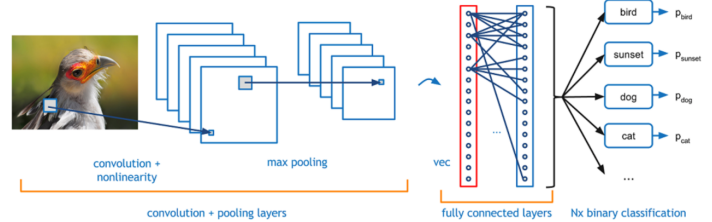
\includegraphics[width=15cm]{images/monografia.png}
    \vspace{0.5cm}
    {\small \textbf{Fonte:} Adaptado de \citeonline{cunha2020redes} \par}
    \label{fig:cnn_architecture}
\end{figure}

\begin{enumerate} 
    \item \textbf{Blocos Convolucionais com Não-Linearidade}
    \begin{itemize}
        \item Segundo \citeonline{pereira2025redes}, cada camada convolucional aplica filtros que detectam padrões locais, seguidos por funções de ativação não lineares como \gls{relu}.
        \item Como observado por \citeonline{pereira2025redes}, camadas iniciais extraem características de baixo nível (bordas, cores), enquanto camadas mais profundas identificam padrões complexos.
    \end{itemize}
    
    \item \textbf{Camadas de Pooling}
    \begin{itemize}
        \item Segundo \citeonline{santos2017abordagem}, a camada de pooling é responsável por reduzir a dimensionalidade dos mapas de características, diminuindo sua largura e altura. Nesse sentido, os autores afirmam que “A operação de pooling possibilita uma invariância espacial. O agrupamento de características, na maioria das arquiteturas de convolução, utiliza uma função de max pooling”.
    \end{itemize}
    \item \textbf{Camadas Totalmente Conectadas}
    \begin{itemize}
        \item \citeonline{utsch2018uso} descreve que uma camada totalmente conectada toma todos os neurônios da camada anterior e os conecta a cada neurônio da camada atual. Em seguida, o autor complementa: “As camadas totalmente conectadas que seguem as camadas convolucionais e de pooling têm por finalidade interpretar essas características de alto nível de abstração, efetuando funções do raciocínio complexo”.
    \end{itemize}
    \item \textbf{Camada de Classificação Binária}
    \begin{itemize}
        \item Conforme \citeonline{utsch2018uso}:
        \begin{citacao}
            Depois das camadas totalmente conectadas, vem a camada de saída. Para o problema de classificação, é comum usar tantos neurônios quanto existam classes a prever, e a saída de cada neurônio tem uma função de ativação de tipo softmax. A softmax é responsável por transformar as saídas dos neurônios em um formato de probabilidades. Isto é, todos os valores são não negativos, menores que um, e o somatório da saída de todos os softmax é igual a 1. Esse formato é necessário para a função de perda cross entropy (entropia cruzada), que é a mais utilizada para os casos de regressão logística, como o é a classificação de imagens (\citeonline[p.~23]{utsch2018uso}).
        \end{citacao}
        \item Embora o trecho citado de \citeonline{utsch2018uso} refira-se a problemas multiclasse (com softmax), em classificação binária, a abordagem padrão é utilizar um único neurônio com ativação sigmóide. Conforme explicado por \citeonline{datacamp_sigmoid}, essa função é amplamente empregada para modelar saídas binárias (e.g., "sim" ou "não"), transformando a combinação linear das features em um valor de probabilidade entre 0 e 1. Essa saída probabilística é compatível com a função de perda binary cross-entropy, otimizando a distinção entre duas classes.
    \end{itemize}
\end{enumerate}

\section{Métricas de Avaliação de Desempenho em Redes Neurais}

Após o treinamento de uma rede neural, torna-se fundamental avaliar seu desempenho por meio de métricas apropriadas, capazes de mensurar sua eficácia em relação aos objetivos da tarefa proposta. Diversas métricas são utilizadas para fornecer uma análise quantitativa e qualitativa dos resultados, conforme discutido por \citeonline{rodrigues2024avaliaccao}, \citeonline{haykin2001redes} e \citeonline{silva2024light}.

\subsection{Matriz de Confusão}

De acordo com \citeonline{silva2024light}, para modelos de classificação, especialmente na abordagem binária, a matriz de confusão é uma das ferramentas mais utilizadas. Ela permite identificar quatro categorias principais que descrevem os acertos e erros do modelo durante a fase de teste:

\begin{itemize}
    \item \textbf{Verdadeiro Positivo (VP)}: instâncias corretamente classificadas como positivas.
    \item \textbf{Falso Positivo (FP)}: instâncias negativas classificadas erroneamente como positivas (erro tipo I).
    \item \textbf{Verdadeiro Negativo (VN)}: instâncias corretamente classificadas como negativas.
    \item \textbf{Falso Negativo (FN)}: instâncias positivas classificadas erroneamente como negativas (erro tipo II).
\end{itemize}

Esses valores servem como base para o cálculo de métricas mais específicas, como acurácia, precisão, revogação, F1-score e AUC-ROC, que oferecem uma análise mais detalhada do desempenho do modelo.

\subsection{Acurácia}

A acurácia é uma métrica amplamente utilizada na avaliação de modelos de classificação, incluindo CNNs \cite{haykin2001redes}. Ela expressa a proporção de predições corretas realizadas pelo modelo em relação ao total de amostras avaliadas.

\begin{equation}
\label{eq:acuracia}
\text{Acurácia} = \frac{VP + VN}{VP + FP + FN + VN}
\end{equation}

Embora forneça uma visão geral do desempenho, a acurácia pode ser enganosa em conjuntos de dados desbalanceados, nos quais há uma disparidade significativa entre o número de amostras por classe \cite{juraszek2014reconhecimento}. Nesses casos, é recomendável utilizar métricas complementares.

\subsection{Precisão}

A precisão (ou \textit{precision}) mede a proporção de verdadeiros positivos entre todas as predições positivas realizadas pelo modelo. É útil quando o custo de falsos positivos é alto.

\begin{equation}
\text{Precisão} = \frac{VP}{VP + FP}
\end{equation}

\subsection{Revogação (Recall)}

A revogação, também chamada de sensibilidade, calcula a proporção de verdadeiros positivos em relação ao total de instâncias que realmente pertencem à classe positiva. Essa métrica é relevante quando o custo de falsos negativos é elevado.

\begin{equation}
\text{Recall} = \frac{VP}{VP + FN}
\end{equation}

\subsection{F1-Score}

O F1-score é a média harmônica entre precisão e revogação. É especialmente útil em cenários onde há necessidade de equilibrar os impactos de falsos positivos e falsos negativos.

\begin{equation}
\text{F1-Score} = 2 \cdot \frac{\text{Precisão} \cdot \text{Recall}}{\text{Precisão} + \text{Recall}}
\end{equation}

\subsection{AUC-ROC}

A métrica AUC-ROC (Área sob a Curva ROC) avalia a capacidade do modelo de distinguir entre classes positivas e negativas. Quanto maior a área sob a curva, melhor o desempenho do modelo em termos de discriminação \cite{rodrigues2024avaliaccao}.

\section{Tipos de Classificação em Redes Neurais}

\subsection{Introdução}
A classificação é uma das tarefas centrais em aprendizado supervisionado, sendo responsável por atribuir rótulos às entradas com base em padrões aprendidos durante o treinamento \citeonline{castro2011aprendizado}. Em redes neurais, essa tarefa é geralmente realizada na camada de saída, que define a estrutura final do modelo de acordo com o tipo de classificação desejado.

\subsection{Classificação Binária}

Neste tipo de problema, o modelo decide entre duas classes distintas, como "positivo" ou "negativo". A saída da rede geralmente consiste em um único neurônio com função de ativação sigmóide, que retorna um valor entre 0 e 1 representando a probabilidade de pertencimento a uma das classes. Esse tipo de estrutura é amplamente utilizado em tarefas como detecção de fraudes, diagnósticos médicos e classificação de sentimentos \citeonline{rossi2015classificacao}. 

A função sigmóide é especialmente adequada para esse tipo de tarefa por produzir uma saída contínua entre 0 e 1, o que facilita a interpretação probabilística do resultado \citeonline{datacamp_sigmoid}.




\subsection{Classificação Multiclasse}

A classificação multiclasse envolve mais de duas categorias mutuamente exclusivas. A camada de saída da rede neural possui múltiplos neurônios, cada um representando uma classe, e utiliza a função de ativação softmax para normalizar as probabilidades. Esse tipo de problema pode ser tratado como uma extensão da classificação binária, em que cada exemplo é atribuído exclusivamente a uma única classe \citeonline{google_multiclasse}. Como destacado pela Google Developers, "o processo pode ser repetido para cada uma das classes originais" \citeonline{google_multiclasse}.

Uma abordagem comum para problemas multiclasse é a decomposição em múltiplos classificadores binários. Por exemplo, em um cenário com três classes (A, B e C), pode-se construir um classificador binário que diferencie entre A+B e C, seguido por outro que distinga entre A e B. Essa técnica é conhecida como estratégia de um-contra-todos (one-vs-rest) ou um-contra-um (one-vs-one), dependendo da forma como os pares de classes são organizados \citeonline{google_multiclasse}.

Um exemplo clássico de aplicação é o reconhecimento de dígitos manuscritos, em que o modelo recebe uma imagem e deve identificar qual número de 0 a 9 está representado.

\subsection{Classificação Multiclasse Um contra Um}

Este tipo de classificação é utilizado principalmente para detecção de anomalias, sendo o modelo treinado exclusivamente com dados de uma classe considerada normal. O objetivo é identificar desvios ou padrões incomuns que não se encaixam na distribuição aprendida. Embora o foco desta classificação seja diferente da abordagem multiclasse, técnicas como o método um contra um também ilustram como modelos binários podem ser adaptados para cenários mais complexos. Segundo a documentação da Microsoft, "mesmo algoritmos de classificação binária podem ser adaptados para tarefas de classificação de várias classes por meio de diversas estratégias" \citeonline{microsoft_onevsone}. Essa flexibilidade é essencial para lidar com problemas em que os dados de classes anômalas são escassos ou inexistentes.

\subsection{Funções de Ativação e de Perda}

A escolha adequada das funções de ativação e de perda é essencial para o desempenho e a capacidade de generalização dos modelos de aprendizado de máquina. As funções de ativação são responsáveis por introduzir não-linearidade nas redes neurais, permitindo que o modelo aprenda padrões complexos nos dados. Já as funções de perda orientam o processo de otimização, indicando o quão distante a predição está do valor esperado \citeonline{iaexpert2020ativacao}. Em tarefas de classificação binária, a função sigmoide é amplamente utilizada por sua capacidade de mapear valores reais para o intervalo $[0, 1]$, permitindo interpretar a saída como uma probabilidade. Sua formulação matemática é dada por:

\begin{equation}
\sigma(x) = \frac{1}{1 + e^{-x}},
\end{equation}

sendo uma função não linear que possibilita ao modelo aprender relações complexas entre os dados. Conforme discutido por \citeonline{gaio2022analise}, a função sigmoide apresenta comportamento assintótico, convergindo para 1 em entradas muito positivas e para 0 em entradas muito negativas, o que reforça sua aplicabilidade em cenários de decisão binária.

Por outro lado, em problemas de classificação multiclasse, a função \textit{softmax} é mais apropriada, pois transforma o vetor de saídas em uma distribuição de probabilidade sobre as classes. Sua expressão é dada por:

\begin{equation}
\text{softmax}(z_i) = \frac{e^{z_i}}{\sum_{j=1}^{K} e^{z_j}},
\end{equation}

onde $K$ representa o número total de classes e $z_i$ é o valor da saída para a classe $i$. A função \textit{softmax} é geralmente combinada com a função de perda de entropia cruzada categórica, que penaliza fortemente previsões incorretas e acelera o processo de convergência durante o treinamento.

\section{Teste de Software em Jogos Digitais}

Os testes de software em jogos digitais apresentam desafios únicos em comparação com aplicações convencionais, devido à complexidade dos sistemas interativos, à imprevisibilidade do comportamento do jogador e à necessidade de garantir uma experiência fluida e imersiva. Segundo \citeonline{costa2024testes}, a automação desses testes tem se mostrado uma alternativa promissora para lidar com essas dificuldades, especialmente em tarefas repetitivas como verificação de colisões, detecção de bugs gráficos e validação de regras de jogo. O estudo bibliográfico conduzido pelo autor destaca que, embora ainda haja limitações na cobertura de testes automatizados em ambientes altamente dinâmicos, ferramentas específicas para jogos têm evoluído significativamente, permitindo maior confiabilidade e eficiência no processo de desenvolvimento. Dessa forma, a adoção de estratégias automatizadas contribui não apenas para a melhoria da qualidade do produto final, mas também para a redução de custos e tempo de produção.

\subsection{Classificação dos testes de software}

Os testes de software podem ser classificados em diferentes categorias, conforme o objetivo e o escopo de cada abordagem. Essa organização é fundamental para garantir a qualidade do produto final, permitindo que diferentes aspectos do sistema sejam avaliados de forma sistemática. Segundo \citeonline{costa2024testes}, os principais tipos de testes incluem:

\begin{itemize}
    \item \textbf{Testes unitários}: verificam o comportamento de unidades individuais de código, como funções ou classes, assegurando que cada componente funcione corretamente de forma isolada.
    
    \item \textbf{Testes de integração}: avaliam a interação entre os componentes do sistema, garantindo que funcionem corretamente quando combinados.
    
    \item \textbf{Testes de sistema}: analisam o comportamento do sistema como um todo, verificando se ele atende aos requisitos definidos.
    
    \item \textbf{Testes de aceitação}: verificam se o sistema atende às expectativas e necessidades do usuário final.
    
    \item \textbf{Testes de desempenho}: medem aspectos como velocidade, escalabilidade e capacidade de resposta do sistema.
    
    \item \textbf{Testes de segurança}: identificam vulnerabilidades e ameaças, garantindo que o sistema esteja protegido contra acessos indevidos.
    
    \item \textbf{Testes de usabilidade}: avaliam a experiência do usuário, considerando fatores como facilidade de uso e interação com a interface.
    
    \item \textbf{Testes de compatibilidade}: verificam se o sistema funciona corretamente em diferentes plataformas, navegadores e dispositivos.
\end{itemize}

Essa classificação contribui para uma abordagem mais eficiente e estruturada no processo de teste, especialmente em contextos complexos como o desenvolvimento de jogos digitais.

\subsection{Estratégias de teste}

A definição de estratégias de teste é essencial para orientar como os testes serão conduzidos ao longo do desenvolvimento de um sistema. Elas estabelecem diretrizes que ajudam a selecionar as técnicas mais adequadas, os recursos necessários e o nível de profundidade das análises. De acordo com \citeonline{costa2024testes}, essas estratégias podem ser classificadas em diferentes abordagens, cada uma com objetivos específicos:


\begin{itemize}
    \item \textbf{Testes caixa-preta}: analisam o comportamento do sistema sem considerar sua estrutura interna. Essa abordagem concentra-se nas entradas e saídas, sendo eficaz para verificar se os requisitos funcionais estão sendo corretamente atendidos.
    
    \item \textbf{Testes caixa-branca}: avaliam o funcionamento interno do sistema, incluindo a lógica de programação e a estrutura de dados. Essa estratégia permite examinar o fluxo de controle, a cobertura de código e a integridade dos componentes internos.
    
    \item \textbf{Testes caixa-cinza}: combinam elementos das abordagens caixa-preta e caixa-branca, possibilitando uma análise mais completa do sistema, tanto em relação ao seu comportamento externo quanto à sua estrutura interna.
    
    \item \textbf{Testes caixa-verde}: são voltados para requisitos específicos, como desempenho, segurança ou usabilidade. Essa estratégia é aplicada para validar características não funcionais que impactam diretamente na qualidade do produto final.
\end{itemize}

A escolha da estratégia mais adequada depende do contexto do projeto, dos objetivos dos testes e das particularidades do sistema em desenvolvimento. No caso de jogos digitais, por exemplo, estratégias como os testes caixa-verde e caixa-preta são especialmente relevantes para garantir uma experiência satisfatória ao usuário e o cumprimento dos requisitos de desempenho.

\subsection{Fases do ciclo de vida de teste}

O teste de software é composto por diversas fases que acompanham o ciclo de desenvolvimento, sendo planejadas desde os estágios iniciais do projeto. Segundo \citeonline{pereira2013beneficios}, uma abordagem eficaz para estruturar essas fases é o modelo de desenvolvimento em “V”, no qual as atividades de teste são integradas às etapas de desenvolvimento, permitindo maior controle de qualidade e identificação precoce de falhas. Esse modelo é ilustrado na Figura~\ref{fig:v}, que demonstra como cada fase de desenvolvimento possui uma etapa correspondente de teste, reforçando a importância da validação contínua ao longo do processo.

\begin{figure}[H]
    \centering
    \caption{Modelo de desenvolvimento em V.}
    \vspace{0.5cm}
    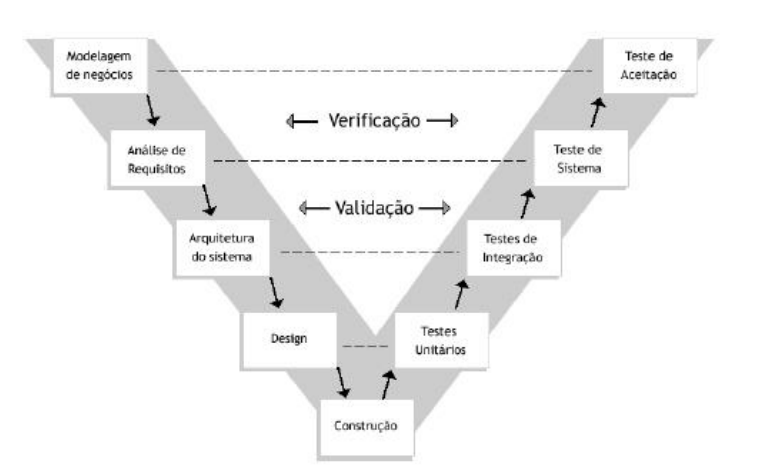
\includegraphics[width=12cm]{images/v.png}
    \vspace{0.4cm}
    {\small \textbf{Fonte:} \citeonline{pereira2013beneficios}}
    \label{fig:v}
\end{figure}

A primeira fase é o \textbf{teste de unidade}, que tem como objetivo verificar se cada módulo ou componente do software atende às especificações definidas no projeto detalhado. Após essa etapa, os módulos são integrados conforme a arquitetura do sistema, iniciando o \textbf{teste de integração}, que busca identificar falhas na comunicação entre os componentes.

Com os subsistemas validados, realiza-se o \textbf{teste de sistema}, que avalia o comportamento do software como um todo, incluindo componentes de hardware e software, com o intuito de verificar se os requisitos funcionais estão sendo atendidos. Em seguida, são aplicados os \textbf{testes de aceitação}, geralmente conduzidos pelo cliente, com o objetivo de validar se o sistema satisfaz os requisitos definidos na fase de especificação.

Por fim, os \textbf{testes de regressão} são executados principalmente durante a fase de manutenção, com o propósito de garantir que modificações realizadas em partes do sistema não tenham introduzido erros em funcionalidades já existentes. Essas fases, quando bem estruturadas e aplicadas, contribuem significativamente para a confiabilidade e qualidade do produto final.

\subsection{Testes no contexto dos jogos digitais}

Embora o ciclo de vida de testes siga princípios semelhantes em diferentes tipos de software, os jogos digitais apresentam desafios específicos que exigem abordagens adaptadas. Em projetos desenvolvidos com motores como o Unity, o teste não deve ser encarado como uma etapa isolada, mas sim como um processo contínuo que permeia todas as fases do desenvolvimento \citeonline{unity2023testing}.

Segundo \citeonline{unity2023testing}, é essencial realizar testes desde os protótipos iniciais até as versões finais, incluindo cada atualização do jogo. Isso envolve não apenas testes funcionais, mas também avaliações de desempenho, experiência do usuário e compatibilidade entre plataformas. O objetivo é garantir que o jogo funcione de forma fluida, sem travamentos, artefatos visuais ou falhas de jogabilidade que possam comprometer a experiência do jogador.

Além dos testes tradicionais, os jogos digitais demandam:

\begin{itemize}
    \item \textbf{Testes de jogabilidade}: Avaliam se as mecânicas do jogo são intuitivas, equilibradas e divertidas \citeonline{unity2023testing}.
    \item \textbf{Testes de compatibilidade}: Verificam o funcionamento do jogo em diferentes dispositivos, sistemas operacionais e resoluções de tela \citeonline{unity2023testing}.
    \item \textbf{Testes de desempenho}: Medem taxa de quadros (FPS), consumo de memória, aquecimento de dispositivos e tempo de carregamento \citeonline{unity2023testing}.
    \item \textbf{Testes de localização}: Garantem que o conteúdo esteja corretamente traduzido e adaptado para diferentes regiões \citeonline{unity2023testing}.
    \item \textbf{Testes com jogadores reais}: Conhecidos como \textit{player testing}, são fundamentais para coletar feedback direto do público-alvo e ajustar o jogo conforme suas expectativas \citeonline{unity2023testing}.
\end{itemize}

Essas práticas não apenas aumentam a qualidade técnica do produto, mas também fortalecem a reputação do estúdio e a fidelidade dos jogadores. Como destaca \citeonline{unity2023testing}, “um único bug pode transformar empolgação em frustração”, tornando o teste uma etapa estratégica no desenvolvimento de jogos digitais.

\section{Trabalhos Correlatos}

